\documentclass[]{article}

%opening
\title{The effects of attitudes towards risk and ambiguity on educational investment: Preliminary results}
\author{Chau Pham}
%\date{} for no date shown
\usepackage{amsmath, amsfonts, amssymb, amsthm, mathtools, mathrsfs}
\usepackage[margin = 1.0in]{geometry}
\usepackage{bbold, soul}
\usepackage{tgpagella}
\usepackage{braket, setspace, parskip, enumitem}
\usepackage[colorlinks, citecolor = blue]{hyperref}
\usepackage[nameinlink, noabbrev]{cleveref}
\usepackage{caption}
\usepackage{threeparttable, makecell, cellspace, multirow, booktabs}
\usepackage{verbatim}
\usepackage{natbib}
\usepackage[bottom]{footmisc}

%---- Simple table template
\begin{comment} 
	\begin{table}[!htbp]\centering
		\begin{threeparttable}
			\setlength{\extrarowheight}{0.2em}
			\begin{tabular}
				content...
			\end{tabular}
			%\caption{text}
			%\label{key}
		\end{threeparttable}
	\end{table}
\end{comment}

%\setlist[enumerate]{label=(\roman*)}

%\setlength{\parindent}{0pt}

\captionsetup[figure]{labelfont=bf}
\captionsetup[table]{labelfont=bf}

\begin{document}

\maketitle
\onehalfspacing

\section{Data \& methodology}
I use data from the Longitudinal Internet Studies for the Social Sciences (LISS panel), which is representative of the Dutch population, and the American Life Panel (ALP), which is representative of the American population. Both datasets contain administrative data as well as survey questions designed for the elicitation of risk and ambiguity attitudes.\footnote{For LISS panel, survey number 44 contains said questions on risk and ambiguity. The ALP counterpart is survey number 243.}

\subsection{Survey questions on risk and ambiguity}
To elicit ambiguity aversion, \citet{DIMMOCK2016559, dimmock2016ambiguity} designed special surveys as part of ALP and LISS panel respectively. Specifically, each individual are asked whether they prefer the risky box, the ambiguous box or either (meaning indifferent) as in \Cref{fig:1}.

\begin{figure}[!ht]
	\setlength{\fboxrule}{1.5pt}
	\setlength{\fboxsep}{0pt}
	\fbox{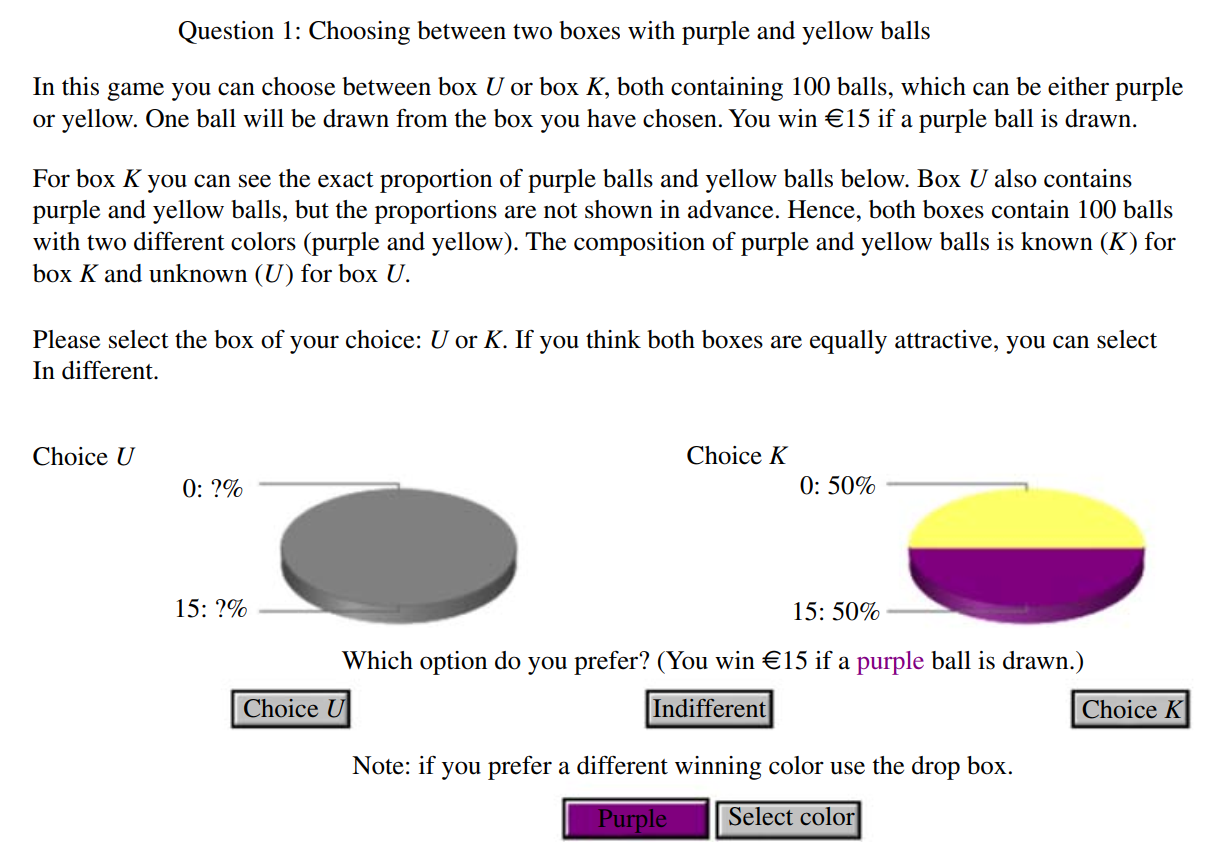
\includegraphics[width=\linewidth]{Figure/figure-1.png}}
	\caption{Question 1 in the ambiguity sequence of the LISS panel.}
	\label{fig:1}
\end{figure}

The question will be asked repeatedly until the respondent chooses "Indifferent" or until the 6th iteration whichever occurs first. \Cref{fig:1} shows the first question in the sequence. If the respondent chooses "Choice U" in this question, she is then presented with a similar question wherein Choice U stays the same while the number of the winning balls in Choice K increases using a bisection method.\footnote{After each question that the respondent chooses either "Choice K" or "Choice U", the proportion of the winning balls in the risky choice is adjusted as follows. In the first question, if "Choice K" is chosen, the proportion of winning ball in the next question is then $(0\% + 50\%)/2 = 25\%$ and $50\%$ becomes the new ceiling instead of $100\%$. If "Choice U" is chosen, the proportion of winning ball in the next question is $(50\% + 100\%)/2 = 75\%$ and $50\%$ becomes the new floor. The new floor and ceiling are carried to the next question and get updated again depending on the subsequent choices of the respondent.} If, on the other hand, "Choice K" is chosen in the first question, in the following question, the number of winning balls in Choice K is reduced. If "Indifferent" is chosen at any stage of the sequence, the sequence stops and the proportion of winning balls in the last stage indicates probability of winning a risky `lottery' that makes the risky choice and ambiguous choice equally attractive. Finally, if "Indifferent" is never chosen, the sequence stops after the 6th iteration of the question and the final probability of winning a risky `lottery' is adjusted via the bisection method. In total, three sequences of questions on ambiguity with varying initial degree of risk are asked in both the LISS panel and ALP.

In a similar manner, to elicit risk attitudes, two sequences of questions about two choices involving sure gain on one side and a risky lottery on the other are presented to respondents. \Cref{fig:2} shows the first question in this sequence of questions on risk for the ALP. Depending on the choices of the respondent, the prize of the sure-gain Box A is updated via a bisection method while the risky Box B remains the same. The question is repeated until "Indifferent" is chosen or until the 4th iteration is reached.

\begin{figure}[!ht]
	\setlength{\fboxrule}{1.5pt}
	\setlength{\fboxsep}{0pt}
	\fbox{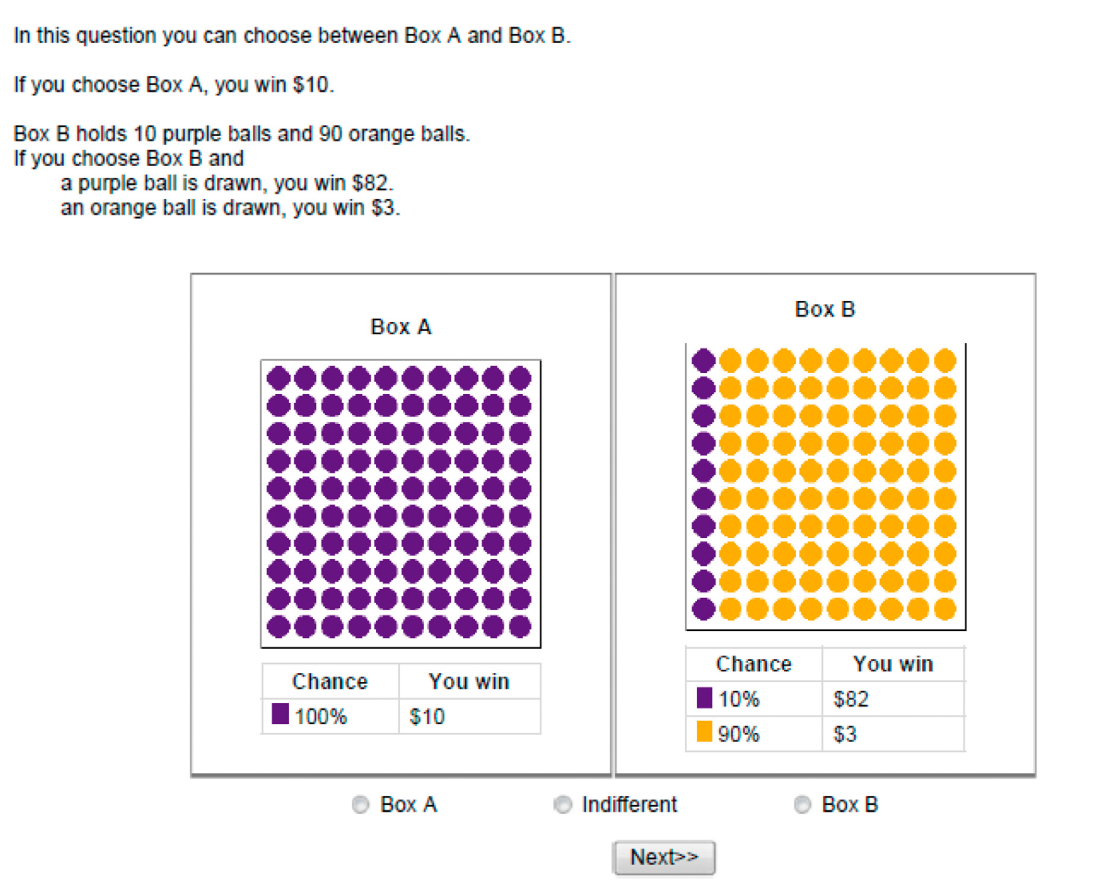
\includegraphics[width = \linewidth]{Figure/figure-2.png}}
	\caption{A randomized question in the risk sequence of ALP.}
	\label{fig:2}
\end{figure} 


\subsection{Elicitation of attitudes towards ambiguity}
The elicitation procedure in both panels follow the source method of \citet{abdellaoui2011} which subsume a variety of models of ambiguity, including prospect theory \citep{tversky1992advances}, Choquet expected utility \citep{schmeidler1989subjective}, and multiple priors \citep{gilboa1989maxmin}. The source method measures ambiguity attitudes via \textit{matching probabilities}, that is, in the context of ALP and LISS ambiguity sequence, the proportion of winning balls in the final iteration. Matching probability can be denoted as follows,
\[m(p)=X/100,\]
where $p$ is the proportion of winning balls when the number of balls of any one colour is the same, $X$ the number of winning balls after the final iteration is reached, and $m(p)$ the \textit{matching probability} of the ambiguity-neutral probability of $p$. If $m(p)<p$, the respondent is ambiguity-averse as she underweigh the ambiguity-neutral probability of the risky choice due to the ambiguous box. By contrast, under ambiguity-seeking, $m(p)>p$. For instsance, in an urn with $100$ balls of 2 colours, $m(0.5)=0.45$ means that the respondent is indifferent between gambling on one colour from the known urn with $45$ of the 100 balls in the known urn of that colour versus an unknown urn containing 100 balls of 2 colours in unknown proportions.   

As shown in \citet{dimmock2016ambiguity}, with the matching probabilities $m(p)$ and $p$, the global ambiguity attitude indices of \citet{abdellaoui2011} can be measured. First, perform a recoding to find the best fitting line between $m(p)$ and $p$, say
\[p\mapsto c+sp \]
with $c$ the intercept and $s$ the slope. The ambiguity indices are defined
\begin{equation}
	a= 1-s\quad\text{(index of ambiguity-generated likelihood insensitivity)}
\end{equation}
and
\begin{equation}
	b = 1-s-2c\quad\text{(index of ambiguity aversion or pessimism).}
\end{equation}
Index $a$ captures \textit{likelihood insensitivity}, defined as the lack of influence of the updating of probabilities following the arrival of new information. Index $b$ captures the degree of \textit{pessimism}, that is, good outcomes are assigned lower weights due to the presence of ambiguity.

\subsection{Elicitation of attitudes towards risk}
Following method described in \citet{tanaka2010, abdellaoui2011}, attitudes towards risk is elicited using expected utility theory (EU) assuming a power utility function, i.e., $u(x)=x^\sigma$.\footnote{An alternative to EU theory is prospect theory \citep{tversky1992advances} with Prelec's \citeyearpar{prelec1998probability} probability weighting function. Prospect theory is adopted in both \citet{tanaka2010, abdellaoui2011} instead of standard EU theory. Due to complications in the calculation of involved parameters, I have not adopted this approach in the following results.} Using two sequences of risk question, the coefficient of relative risk aversion (CRRA) can be estimated by fitting the data to the reduced-form regression:
\begin{equation}
	\log(CE)={1\over \sigma}\log(p) + \beta\times \log(stake).
\end{equation}
and $\rho=1-\sigma$ is the estimated CRRA coefficient.


\section{Preliminary results}
\subsection{LISS panel}

% Table created by stargazer v.5.2.3 by Marek Hlavac, Social Policy Institute. E-mail: marek.hlavac at gmail.com
% Date and time: Mon, Jun 26, 2023 - 16:22:59
\begin{table}[!htbp] \centering 
  \caption{Summary Statistics (LISS)} 
  \label{} 
\begin{tabular}{@{\extracolsep{5pt}}lccccc} 
\\[-1.8ex]\hline 
\hline \\[-1.8ex] 
Statistic & \multicolumn{1}{c}{N} & \multicolumn{1}{c}{Mean} & \multicolumn{1}{c}{St. Dev.} & \multicolumn{1}{c}{Min} & \multicolumn{1}{c}{Max} \\ 
\hline \\[-1.8ex] 
Monthly school fees (euros) & 161 & 105.484 & 317.641 & 0 & 3,200 \\ 
Financial responsibility & 161 & 0.522 & 0.501 & 0 & 1 \\ 
Education & 148 & 2,986.588 & 1,156.707 & 500 & 7,000 \\ 
Household income & 161 & 2.513 & 8.948 & $-$4.836 & 38.579 \\ 
Risk aversion ($\rho$) & 161 & $-$0.101 & 0.219 & $-$0.872 & 0.075 \\ 
$AA_{0.1}$ & 161 & 0.091 & 0.218 & $-$0.469 & 0.469 \\ 
$AA_{0.5}$ & 161 & 0.606 & 0.304 & $-$0.072 & 0.875 \\ 
$AA_{0.9}$ & 161 & $-$0.005 & 0.523 & $-$1.184 & 1.184 \\ 
Index $a$ & 161 & 0.617 & 0.292 & 0.096 & 1.942 \\ 
\hline \\[-1.8ex] 
\end{tabular} 
\end{table} 


% Table created by stargazer v.5.2.3 by Marek Hlavac, Social Policy Institute. E-mail: marek.hlavac at gmail.com
% Date and time: Mon, Jun 26, 2023 - 23:00:23
\begin{table}[!t] \centering 
  \caption{Simple regression models} 
  \label{tab:2} 
  \begin{threeparttable}
\begin{tabular}{@{\extracolsep{5pt}}lcc} 
\\[-1.8ex]\hline 
\hline \\[-1.8ex] 
 & \multicolumn{2}{c}{\textit{Dependent variable:}} \\ 
\cline{2-3} 
\\[-1.8ex] & \multicolumn{2}{c}{Monthly schooling fees} \\ 
\\[-1.8ex] & (1) & (2)\\ 
\hline \\[-1.8ex] 
 $AA_{0.1}$ & $-$173.124 &  \\ 
  & (162.102) &  \\ 
  & & \\ 
 $AA_{0.5}$ & 348.757$^{**}$ &  \\ 
  & (155.031) &  \\ 
  & & \\ 
 $AA_{0.9}$ & $-$108.627 &  \\ 
  & (100.394) &  \\ 
  & & \\ 
 Index $a$ &  & $-$15.339 \\ 
  &  & (55.538) \\ 
  & & \\ 
 Index $b$ &  & $-$156.234 \\ 
  &  & (97.667) \\ 
  & & \\ 
 Risk aversion & $-$2.264 & $-$1.499 \\ 
  & (3.479) & (3.534) \\ 
  & & \\ 
 Household income & $-$0.002 & 0.003 \\ 
  & (0.026) & (0.026) \\ 
  & & \\ 
 \# of living-at-home children & 77.571$^{**}$ & 77.813$^{**}$ \\ 
  & (37.732) & (38.383) \\ 
  & & \\ 
\hline \\[-1.8ex] 
Controls and constant & YES & YES \\ 
Observations & 148 & 148 \\ 
R$^{2}$ & 0.112 & 0.080 \\ 
Adjusted R$^{2}$ & 0.025 & $-$0.002 \\ 
Residual Std. Error & 326.065 (df = 134) & 330.679 (df = 135) \\ 
F Statistic & 1.296 (df = 13; 134) & 0.972 (df = 12; 135) \\ 
\hline 
\hline \\[-1.8ex] 
\end{tabular} 
\begin{tablenotes}[flushleft]
	\footnotesize
	\item \textit{Note:} $^{*}p<0.1$; $^{**}p<0.05$; $^{***}p<0.01$
	\item Control variables include Education, a dummy for financial responsibility and another dummy for possession of a PC at home.
\end{tablenotes}
\end{threeparttable}
\end{table} 


LISS panel has a total of more than 13,000 participants. Of which, 1,935 completed the surveys on ambiguity and risk. To match data on attitudes and educational investment, I merge the survey on ambiguity with another on time use. Data for time use and consumption surveys  are collected in many waves but it was not until Wave 6 that a question on the specific amount of monthly schooling expense was asked. As the ambiguity survey was conducted in January, 2010 while data of Wave 6 of the Time use and consumption survey was collected in November, 2019, the time discrepancy calls for great caution when interpreting the results of any inference made. An assumption that will be made here is the invariability of attitudes towards risk and ambiguity over time. Summary statistics of the sample of LISS panel are reported in \Cref{tab:1}. 

The results of two simple regression models are reported in \Cref{tab:2}. 

\subsection{American Life Panel}
I haven't been able to progress much with ALP due to some difficulties when extracting data and calculating parameters of ambiguity and risk aversion. 

\pagebreak

\bibliographystyle{apalike}
\bibliography{bibliography.bib}

\end{document}
